 %!TEX root = Memoria_TFM.tex
\section{Anti-spoofing and biometrics systems}
At the same time as technology advance, capture systems and processing algorithms have proceed too. This open an immense options quantity and one of them is the capability of developing more sophisticated identification systems, giving way to biometrics systems.\\

\subsection{Historical introduction}
There were in the 1870s when the necessity of identifying people getting physical characteristics appeared. Alphonse Bertillon had the desire of identifing jail prisoners, in order to do that, the skull diameter, arm and foot length were utilized for that purpose in USA until the 1920s \cite{Intro_biometrics}.\\

There were in the 1880s when fingerprint and facial identification were proposed. With the appearance of digital signals processing systems in 1960, the voice and the fingerprint biometric systems were started to be investigated and researches started to think to use this system to identification in access control security \cite{Intro_biometrics}.\\
 
Ten years later, the geometry of the hand was started to be a area of interest for automated technologies of identification. The retina and signature verification appeared in the 80s and after a short time the face systems \cite{Intro_biometrics}.\\

The last biometrics systems appeared in the 1990s with the iris recognition \cite{Intro_biometrics}.\\

\subsection{Biometrics}
Biometrics is a characteristics that each human own, is inherent and is exclusive for each human. Because of that, are used as identification.\\

Biometrics could be distinguished as physical or behavioural biometrics. Physical biometrics are characteristics which every human is born with, is genetic, fingerprint, face, DNA, ear and iris are physical biometrics; behavioural biometrics are characteristics which has been matured with person, is  psychological, signature and gait are behavioural biometrics \cite{biometrics_beha}.\\

Nowadays, the quantity of biometrics is considerable. There are not a biometric which is only used or could be selected as optimal, although fingerprint is the most popular biometrics \cite{2d_3d_face}. The characteristic of each biometrics makes it appropriate for the application \cite{Intro_biometrics}.\\% The most common biometrics are described \cite{Intro_biometrics}:

%\begin{description}[noitemsep,topsep=8pt,parsep=0pt,partopsep=20pt] \item \textbf{DNA:} using the DNA for recognition is widely used in forensic. This biometric is intrusive and identical twins share the ADN \cite{Intro_biometrics}. \end{description}

%\subsubsection{Face biometric}
%The thesis research is focused on face biometric.\\

\subsection{Biometric system}
A biometric system could be defined as a structure which collect determined biometric data from a user. The input data is processed in order to obtain features with which are compared with template samples. A biometric system could be labelled as a recognition system or verification system depending on the realized task \cite{Intro_biometrics2}:
\begin{description}[noitemsep,topsep=8pt,parsep=0pt,partopsep=20pt]
\item \textbf{Verification system:} user claims an identity and the system validates the identity comparing the acquired data with the stored in the template database.
\item \textbf{Recognition or Identification system:} user data is compared with the all the template database to find user's identity. The identity is not claimed by the user and is given by the system in function of features. 
\end{description}

\begin{figure}[htb]
\centering
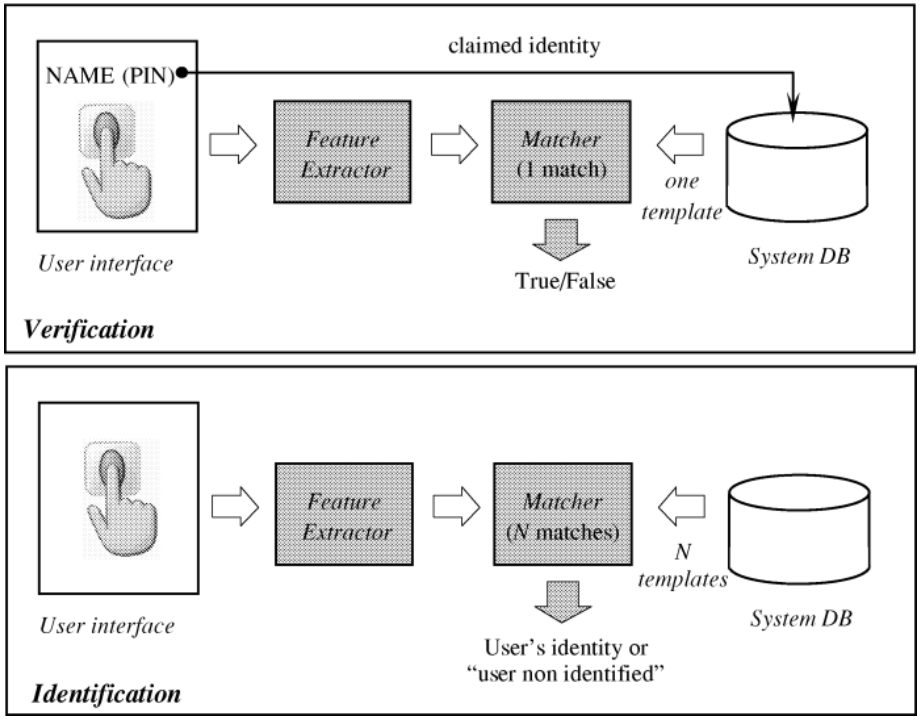
\includegraphics[width=0.5\textwidth]{images_miscelaneus/verif_identif.PNG}
\caption{Verification and Identification system diagram. Image obtained from \cite{Intro_biometrics2}} \label{fig:Verif_ident}
\end{figure}

Figure \ref{fig:Verif_ident} (figure obtained from \cite{Intro_biometrics2}) represents briefly the process of the acquired data until be compared  with the system database if it is a verification or recognition system. The modules showed in figure \ref{fig:Verif_ident} are described \cite{Intro_biometrics2}: 
\begin{description}[noitemsep,topsep=8pt,parsep=0pt,partopsep=20pt]
\item \textbf{Sensor:} the first module is the sensor, which obtain the user's biometric. Depending on the biometrics, the sensor can vary greatly.
\item \textbf{Feature extractor:} input data is processed to obtain the features. The features that are extracted in this module should be the same as the saved in the database.
\item \textbf{Matcher:} features obtained from the previous module are compared or classify with the templates database so the identity of the user could be verified or assigned.
\item \textbf{Database:} the database is formed by templates which are going used as true samples to compare the obtained with sensors. An user should be registered to the system contributing with it biometric template. 
\end{description}

\subsection{Spoofing}
As the same time as biometrics authentication systems appeared, the attacks to trick systems emerge and they are called \textit{spoofing attacks}. For example making plaster molds for geometric hand biometrics or fingerprints would be an attack as the presented in figure \ref{fig:Spoof_fingerprint} (image obtained from \cite{fingerprint_image}).\\

\begin{figure}[htb]
\centering
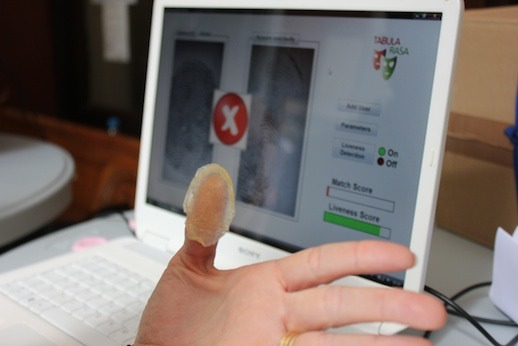
\includegraphics[width=0.5\textwidth]{images_miscelaneus/spoofing_fingerprint.jpg}
\caption{Spoofing fingerprint. Image obtained from \cite{fingerprint_image}} \label{fig:Spoof_fingerprint}
\end{figure}

Spoofing is referenced to impersonate a biometric system trying to be verified or get a identity when user is not a genuine. The attack would depend on the biometry and the capturing system \cite{Spoofing_survey}. Attacks are usually made with artificial articles.\\

In order to get the tricks and do not allow spoofing attacks, \textit{anti-spoofing} tries to minimize the attacks or prevent them.\\

Anti-spoofing algorithms could be distinguish depending on the biometric system module which is combined \cite{Spoofing_survey}:
\begin{description}[noitemsep,topsep=8pt,parsep=0pt,partopsep=20pt]
\item[Sensor level:] extra equipment is added to the sensor, the new device is responsible of getting a living attribute as sweat or blood pressure. 
\item[Feature level:] anti-spoofing detection is made after the sample has been acquired. The sample is processed and software decided if it is a genuine or fake user.
\item[Score level:] after the feature extraction, when the scores are obtained, the biometric system decide if user is genuine or not fusing methods. This method is the newest.
\end{description}


Antis-poofing systems and scenarios could be evaluated. Depending on how is evaluated two methoids are distinguised \cite{Spoofing_survey}:
\begin{description}[noitemsep,topsep=8pt,parsep=0pt,partopsep=20pt]
\item[Algorithm-based or technology evaluation:] Evaluate algorithms that prevents anti-spoofing.
\item[System-based or scenario evaluation:] Evaluate the entire acquisition systems including the sensor.
\end{description}

In this project it is going to be developed the algorithm to detect anti-spoofing attacks when face is using as biometrics. Given an image, the system has to decide if it is an attack or a genuine user. It would be a verification task.\\

\subsection{Face anti-spoofing}
Face biometrics is very used biometric system because of its attributes as is not intrusive, it is easy to capture images, it is very accepted by people as biometrics. \\

The principal or main used acquire system are visible light cameras although other cameras as infra-red  or depth camera are used too. Using different types of camera could help to detect anti-spoofing attacks.\\

The disadvantages of cameras as sensor are that the illumination should be controlled and images from differents angles could not be suitable, in addition, people expresions or face occlusions are complicated to work with \cite{survey2,2d_3d_face}. The main advantage of using a visible light camera as sensor is the cost, that is very low. \\

The location of verification or identification system could be in a static and specific place as the office entry or could be a wide place as a subway or an airport \cite{survey2}.\\

Attack to this biometric system is also easy, face images from people are easy to obtain in social networks. The spoofing attacks could be 3D attacks if 3D masks are used or 2D attacks if printed photos, 2D mask or displaying an image or video in a smarthpone or tablet \cite{2d_3d_face}. Moreover, those attacks cost is very low \cite{distorsion}.\\ 

\begin{figure}[htb]
\centering
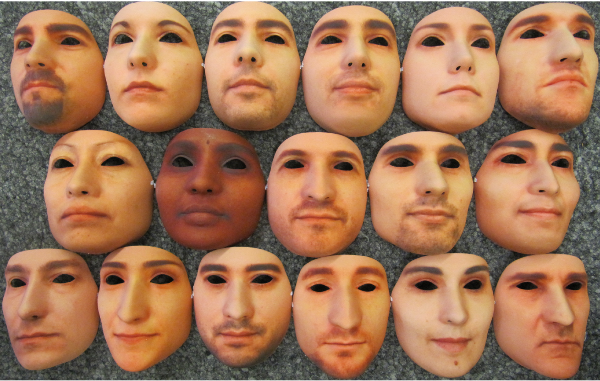
\includegraphics[width=0.5\textwidth]{images_miscelaneus/fig_masks.png}
\caption{3D face masks. Image obtained from \cite{3dmask}} \label{fig:3dMasks}
\end{figure}

In figure \ref{fig:3dMasks} (image obtained from \cite{3dmask}) are represented 3D resin faces mask. This masks are used for a 3D face mask database but could be used as face spoofing attack. 3D mask could be made of silicone too and are cheaper that resin mask.\\

2D mask, printed photos or images or videos displayed in a smart device are attacks easier to obtain thanks to the accessibility to personal information in social networks or the easy purchase of visible light cameras.\\

To argue spoofing attacks, feature level is the most studied method. Literature separates into two groups, dynamic and static approach \cite{Spoofing_survey}:
\begin{description}[noitemsep,topsep=8pt,parsep=0pt,partopsep=20pt]
\item[Dynamic:] is based in motion to detect anti-spoofing, for instance, blink eyes or optical flow assessment, therefore a temporal sequence of images are need. It could be efficient when image attacks are used, but not too accurate when videos are used. 
\item[Static:] a unique image is analysed.
\end{description}

Different techniques to decide if a user is being impersonate are being researched and could be used with image and video sequences \cite{Spoofing_survey}.\\

Texture based methods are one of the most investigate methods. Use Local Binary Patterns (LBP),  Histogram of Oriented Gradients (HOG) or Difference of Gaussian (DoG) algorithms to extract images features \cite{distorsion,Spoofing_survey}.\\

Motion or liveness detection methods search for movement in videos asking user to do something or analysing the frames sequence. The liveness could be detected in blinking eyes, lip movement or head rotation \cite{distorsion,Spoofing_survey}.\\

Others methods, as multispectral-based anti-spoofing, uses images obtained from an alternative to visible light cameras as infra-red cameras \cite{distorsion}.\\
